\documentclass[12pt,a4paper,oneside]{book}
\usepackage[top=2.5cm, bottom=3cm, left=2.5cm, right=2.5cm]{geometry}
\usepackage[utf8]{inputenc}
\usepackage[titletoc,title]{appendix}
\usepackage[linewidth=1pt]{mdframed}
\usepackage{framed}
\usepackage{listings}
\usepackage{smartdiagram}
\usepackage{smartdiagram}
\usesmartdiagramlibrary{additions}
\lstdefinestyle{customc}{
	belowcaptionskip=1\baselineskip,
	breaklines=true,
	frame=L,
	xleftmargin=\parindent,
	language=C,
	showstringspaces=false,
	basicstyle=\footnotesize\ttfamily,
	keywordstyle=\bfseries\color{green!40!black},
	commentstyle=\itshape\color{purple!40!black},
	identifierstyle=\color{blue},
	stringstyle=\color{orange},
}

\lstdefinestyle{customasm}{
	belowcaptionskip=1\baselineskip,
	frame=L,
	xleftmargin=\parindent,
	language=[x86masm]Assembler,
	basicstyle=\footnotesize\ttfamily,
	commentstyle=\itshape\color{purple!40!black},
}

\lstset{escapechar=@,style=customc}

\lstset{
	literate=%
	{à}{{\'a}}1
	{í}{{\'i}}1
	{é}{{\'e}}1
	{è}{{\`e}}1
	{ý}{{\'y}}1
	{ú}{{\'u}}1
	{ó}{{\'o}}1
	{ě}{{\v{e}}}1
	{š}{{\v{s}}}1
	{č}{{\v{c}}}1
	{ř}{{\v{r}}}1
	{ž}{{\v{z}}}1
	{ď}{{\v{d}}}1
	{ť}{{\v{t}}}1
	{ň}{{\v{n}}}1
	{ů}{{\r{u}}}1
	{Á}{{\'A}}1
	{Í}{{\'I}}1
	{É}{{\'E}}1
	{Ý}{{\'Y}}1
	{Ú}{{\'U}}1
	{Ó}{{\'O}}1
	{Ě}{{\v{E}}}1
	{Š}{{\v{S}}}1
	{Č}{{\v{C}}}1
	{Ř}{{\v{R}}}1
	{Ž}{{\v{Z}}}1
	{Ď}{{\v{D}}}1
	{Ť}{{\v{T}}}1
	{Ň}{{\v{N}}}1
	{Ů}{{\r{U}}}1
}
%\usepackage[french]{babel}
%\select@language{french}
\usepackage{hyperref}
\hypersetup{
	colorlinks,
	citecolor=black,
	filecolor=black,
	linkcolor=black,
	urlcolor=black
}
\usepackage{array}
\usepackage{makecell}
\usepackage{gensymb}
\renewcommand\theadalign{cb}
\renewcommand\theadfont{\bfseries}
\renewcommand\theadgape{\Gape[4pt]}
\renewcommand\cellgape{\Gape[4pt]}

\usepackage{fancyhdr}
\renewcommand{\chaptername}{Chapitre}
\usepackage{amsmath}
\usepackage{amsfonts}
\usepackage{amssymb}
\usepackage{color}
\usepackage{caption}
\usepackage{graphicx}
\usepackage{subfig}
\usepackage{float}
\usepackage{amssymb}
\usepackage{framed}
\usepackage{wrapfig}
%\captionsetup[table]{name=Figure}

\usepackage[french,Algorithme]{algorithm}
%\renewcommand{\thealgorithm}{}
\usepackage[noend]{algpseudocode}

\makeatletter
\def\BState{\State\hskip-\ALG@thistlm}
\makeatother

\usepackage{color}

\renewcommand{\bibname}{Bibliographie}
%\usepackage[usenames,dvipsnames]{xcolor}
\newcommand{\HRule}{\rule{\linewidth}{0.5mm}}
\renewcommand{\contentsname}{Table des matières}
%\renewcommand{\listtablename}{Listes des tableaux}
\renewcommand{\listfigurename}{Listes des figures}
\renewcommand{\appendixname}{Annexe}
%\captionsetup[table]{name=tableau}
\renewcommand\thesection{\arabic{section}}
\renewcommand\thesubsection{\thesection.\arabic{subsection}}
\setcounter{secnumdepth}{4}
\usepackage{titlesec}
\titleformat{\paragraph}
{\normalfont\normalsize\bfseries}{\theparagraph}{1em}{}
\titlespacing*{\paragraph}
{0pt}{3.25ex plus 1ex minus .2ex}{1.5ex plus .2ex}

\pagestyle{fancy}
\lhead{\leftmark}
\rhead{}
%\cfoot{center of the footer!}
\renewcommand{\headrulewidth}{0.4pt}
\definecolor{Titre}{rgb}{0.09,0.21,0.36}
\definecolor{Sous-titre}{rgb}{0.31,0.51,0.74}
\usepackage{titlesec}

\begin{document}
	\begin{titlepage}
	
		\begin{center}
			\textsc{\Large \textbf{République Algérienne Démocratique et Populaire}\\[.20cm]
				\vspace*{\stretch{0.02}}
				\Large\textbf{ Ministère de l’Enseignement Supérieur et de la Recherche Scientifique} \\[.20cm]
					\vspace*{\stretch{0.02}}
				\Large \textbf{Université des Sciences et de la Technologie Houari Boumediene \\[.25cm]
					\vspace*{\stretch{0.02}}
					Faculté d'Informatique et d'Électronique \\[.25cm] \vspace*{\stretch{0.02}}
					Département d'Informatique \\ Mémoire en licence }}
			\vspace*{\stretch{0.3}}
			\begin{figure}[h]
				\centering
				
\includegraphics[scale=0.7]{images/USTHB.jpg}
			\end{figure}
			
			\vspace*{\stretch{0.3}}
			\Large \textbf{Option}\\ Licence informatique générale \\ \Large\textbf{Thème}
			% Title
			
			\HRule \\[0.4cm]
			{ \huge \bfseries  }
			\LARGE Émulateur d'un tableau moyennant une Kinect. 
			\HRule \\[1.5cm]
		
			\begin{minipage}{0.5\textwidth}
				\begin{flushleft}
					Sujet proposé par :\\
					
					
					
				\end{flushleft}
				\begin{flushleft}\large
					Mr S.LARABI\\
				\end{flushleft}
				
				\begin{flushleft}\large
				Soutenu le :31/mai/2017
				\end{flushleft}
			\end{minipage}%
			\begin{minipage}{0.5\textwidth}
				\begin{flushright}
					{Réalisé par:}\\
				\end{flushright}
				
				\begin{flushright} \large
					Hassina Safaa \textsc{MOULAI}\\
				\end{flushright}
				
				\begin{flushright} \large
					Nesrine Lilia \textsc{HANED}\\
				\end{flushright}
				
			\end{minipage}
		\begin{flushleft}
			Devant le jury composé de :
		\end{flushleft}	
	
			\Large
			\begin{center}
				
			
				
				
				\begin{tabular}{lll}
					%  \hline
					% after \\: \hline or \cline{col1-col2} \cline{col3-col4} ...
					Mme S. AOUAT      & Présidente & USTHB\\
					Mme D. DAHMANI    & Examinatrice  & USTHB\\
					Mr S.LARABI  & Promoteur   & USTHB\\
					
					% \hline
				\end{tabular}
			\end{center}
			
			\begin{center}
				\textbf{Binôme :115/2017}
			\end{center}
		\end{center}
	\end{titlepage}
	%\renewcommand{\baselinestretch}{1.50}\large
	\pagenumbering{gobble}
	\pagenumbering{gobble}

	\chapter*{Remerciements}
	Nous tenons tout d'abord à remercier dieu le tout puissant et miséricordieux, qui nous a donné la force et la patience d'accomplir ce modeste travail.\\
	En second lieu, nous tenons à remercier Monsieur le professeur Slimane LARABI, notre promoteur, pour ses précieux conseils, son sens de la pédagogie, sa confiance , et pour le temps qu’il nous a consacré.
	Nos vifs remerciements vont également aux membres du jury pour l'intérêt qu'ils ont porté à notre recherche en acceptant d'examiner notre travail et de l'enrichir par leurs propositions.\\
	Enfin, nos plus sincères remerciements vont à nos famille et amis, qui nous ont accompagné, aidé, soutenu et encouragé tout au long de la réalisation de ce mémoire.
	\tableofcontents
	
	
	\listoffigures
	\newpage
	\pagenumbering{arabic}
	
	
	\chapter*{Introduction Générale}
	
	
	
	\addcontentsline{toc}{chapter}{Introduction générale}
	L'informatique visuelle suscite actuellement un large intérêt, et prends une grande part dans le quotidien de l'homme, ce qui se traduit par des projets de recherche  et des applications intelligentes développées et commercialisées en multimédia et jeux sur appareils mobile, en visualisation de données, en analyse d'image et de la vidéo.\\
	
	La vision artificielle, élément de l'informatique visuelle, connaît un développement rapide qui est présent dans notre quotidien. Les caméras, premier éléments de tels systèmes, sont utilisées en vidéo surveillance (dans les magasins, rues ou aéroports), en conduite (aide au guidage ou détection d’obstacles), et bien d’autres applications encore... Pour l’être humain, voir est une action innée et facile , mais  nous ne mesurons souvent pas la difficulté pour obtenir les mêmes performances artificiellement en exploitant des outils de vision. Malgré les avancées de la vision par ordinateur, les systèmes développés sont très loin d’égaler les performances de l’œil et du cerveau humains.\\
	
	L'image de profondeur commence à connaître une multitude d'applications en raison de la richesse d'informations contenue. Un système émulateur d'un mur tactile a été déjà développé par l'équipe de recherche de S. Larabi et qui est en cours de dépôt de brevet d'invention.
	C'est dans le même contexte, le sujet qui nous a été demandé consiste à développer les premiers éléments d'un système informatique d'un tableau pour écriture basé sur l'image de profondeurs. Le système affichera une zone sur écran qui traduira les mouvements d'un stylo sur une surface plane en écriture.\\
	
	Le travail réalisé et présenté dans ce mémoire est scindé en trois chapitres. Nous commençons par un bref état de l'art sur les applications basées sur la kinect. Nous décrivons dans le second chapitre le travail de conception réalisé. Le dernier chapitre est consacré aux résultats obtenus. Nous terminons ce mémoire par une conclusion et les possibilités d'amélioration de ce système.
	
	\chapter{État de l'art}
	
	
	
	\section{Vision artificielle:}
	
	\subsection{L'interaction homme machine}
	L’interaction Homme-Machine repose principalement sur des techniques exploitant des périphériques intermédiaires entre la personne et la machine tels que le clavier, souris, moniteur etc.\\
	Actuellement, la recherche s'est orientée vers de nouveaux concepts. En effet, l’utilisateur doit être en mesure d'interagir avec son environnement et ce en usant de son corps sans aucune contrainte physique. D’ailleurs, certaines parties du corps humain peuvent être considérées comme  des périphériques d’Entrée/Sortie, ce qui rapproche considérablement le monde réel du monde électronique.\\
	Afin d'atteindre cet objectif, une capture du comportement, des mouvements et des interactions observées  de l’utilisateur et de son entourage est nécessaire. C’est là où la perception artificielle entre en jeu.
	
	
	\subsection{Définition de la Vision Artificielle}
	
	La vision par ordinateur est une branche du domaine de l'intelligence artificielle, elle a pour principal objectif de donner la capacité à une machine d'analyser, traiter et comprendre une ou plusieurs images prises par un système d'acquisition, autrement dit elle essaye de réaliser une compréhension d’une scène ou d’un phénomène à partir d’images prises avec une ou plusieurs caméras, mélangeant perception, analyse et contrôle [1].\\
	
	C'est une approche qui consiste à simuler la vision humaine à travers un traitement des données visuelles qui inclut des modèles fondés sur la géométrie, la physique, la biologie, les statistiques et la théorie d’apprentissage.
	
	Grâce à l’évolution de la puissance de calcul des processeurs, la banalisation des dispositifs d’acquisition, l’arrivée de l’interaction homme/machine comme étant une source inépuisable d’expérimentation, la vision par ordinateur s'est largement enrichie, ce qui a multiplié l’ensemble des applications générés et a créé de nouveaux enjeux industriels.
	
	\subsection{Systèmes de Vision Artificielle}
	
	Un système de vision artificielle est un système regroupant un ensemble de processus permettant de reproduire la vision humaine en se servant de capteurs et de processeurs.
	
	Il dispose en entrée des données visuelles (images numériques) et doit fournir en sortie une interprétation de ces dernières.
	
	La donnée visuelle que traite un système de vision artificielle est bidimensionnelle ou tridimensionnelle, ainsi on peut distinguer deux types de système de vision:
	
	\subsubsection{Les systèmes de vision bidimensionnels}
	Ces systèmes n'exploitent pas la notion de profondeur, mais offrent une acquisition de l'image avec deux dimensions seulement. Ces systèmes sont utilisés dans des domaines tels que la télédétection et la reconnaissance de caractères.
	
	\subsubsection{Les systèmes de vision tridimensionnels}
	Ces systèmes exploitent la notion de profondeur, ce qui permet d’obtenir une description en trois dimensions de la scène. Cette profondeur peut être obtenue par différentes techniques. On distingue deux types de systèmes tridimensionnels [2].
	
	\paragraph{Systèmes de vision tridimensionnels actifs}
	
	Les systèmes de vision actifs sont des systèmes utilisant un émetteur et un récepteur, l'émetteur a pour mission d'envoyer  un faisceau d'ondes vers la scène (ondes lumière, sonores), puis la rétro diffusion vers le récepteur va permettre de localiser les objets détectés dans la scène. La mesure du temps d'aller-retour ou de l'intensité du faisceau émise nous permettra aussi de connaître la distance de ces objets par rapport au capteur.
	Les performances de ces systèmes actifs peuvent être réduites par certains problèmes liés à la surface réfléchissante de la cible qui peut absorber le faisceau, le diffuser ou le réfléchir dans d'autres directions.
	
	\paragraph{Systèmes de vision tridimensionnels passifs}
	C’est des systèmes qui utilisent uniquement les images de la scène prises sous des angles différents pour la reconstitution de l’information 3D [2].
	
	Dans le cas de l'utilisation de deux caméras, il s’agit donc de vision stéréoscopique. 
	
	\section{Reconnaissance et détection d'objets:}
	Aussi appelé \textbf{reconnaissance  des  formes}, cette  appellation  désigne  les  méthodes qui à partir de l’observation d’un objet lui attribuent une classe. 
	Par exemple, un système qui, à partir d’une image, classifie des objets volants soit dans une classe avions, soit dans une classe non-avions, réalise une tâche de reconnaissance d’objets.
	
	L’observation d’un objet peut être très différente selon le domaine d’activité dans lequel nous évoluons. Souvent c’est une observation visuelle qui est utilisée (photo, séquence vidéo, image médicale, image satellite, etc.), mais il est également possible d’avoir une analyse radar, laser ou sonore, le champ d’applications étant très large.
	 De même, le motif à reconnaître et à classer peut-être simple ou complexe, et les outils développés sont adaptés à chaque utilisation. Par exemple, un cube sera plus facile à reconnaître qu’un visage car il a des propriétés physiques constantes dans le temps et l’espace  alors qu’un visage est sujet à beaucoup plus de changements [3]. Plusieurs approches existent:
	
	\subsection{Approche 2D}
	Une première approche de la reconnaissance d’objets en trois dimensions est de se baser sur une bibliothèque d’images en deux dimensions. En effet, en considérant plusieurs vues d’un objet en deux dimensions, on peut espérer pouvoir en faire concorder une avec la vue 3D courante. Un des gros avantages du passage par une vue 2D est l’augmentation de la vitesse de calcul.
	
	On peut utiliser pour ce faire un système de reconnaissance de points d’intérêts. Ces mécanismes se servent des variations géométriques de l’objet à reconnaître afin d’observer des similitudes. On y retrouve plusieurs procédés.
	
	La variation de profondeur est aussi utilisée en partant du principe que la caméra est toujours à la même auteur du sol.
	
	\subsection{Approche géométrique}
	
	Comme son nom l’indique, cette méthode se base sur des attributs géométriques des objets à reconnaître. Par conséquent, elle est bien indiquée pour des objets simples (bouteille, livre...) mais sera plus difficile à déployer pour des objets plus complexes (jouets, voiture...).
	Dans cette approche, un objet est décrit à travers un ensemble de paramètres, représenté par des vecteurs.
	
	Afin d’effectuer une classification et obtenir des régions d’intérêt, une phase d’apprentissage est faite pour créer un nuage de point pour chaque type d’objet. On peut alors déterminer des classes d’objets en observant les différentes densités de points (voir figure \ref{fig1n}).
	
	\begin{figure}[H]
		\centering
		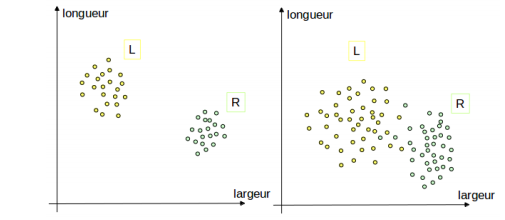
\includegraphics[scale=1]{images/chaptre1.png}
		\caption{Nuage de points représentant les classes d’objets selon leurs caractéristiques.
			A gauche les classes sont sans ambiguïté, à droite les classes sont plus difficile à isoler.}
		\label{fig1n}
	\end{figure}
	
	Une fois que les différentes zones sont mises en évidence, il faut réussir à discriminer les zones entre elles pour faire ressortir les classes d’objets. Enfin, lorsque l’objet à déterminer a été réduit à un ensemble de vecteur, une étude probabiliste permet de déterminer l’appartenance de l’objet à une classe. Comme on peut se douter, plus le nombre de classe est élevé et proche	les une des autres et plus la décision d’appartenance sera délicate à faire [7].
	
	\section{Images de profondeurs et applications}
	
	\subsection{Présentation de la KINECT}
	La Kinect est une caméra 3D créée initialement par Microsoft pour l’industrie des jeux vidéo qui utilise des techniques d'interaction. Ce produit Microsoft conçu en 2008 est issue des deux mots anglais "Kinectic" qui signifie "cinétique" et du mot "connect" qui signifie "connecter". Elle est compatible avec la console de jeu Xbox, et permet de commander cette dernière vocalement à l’aide de microphones et par gestes grâce à la reconnaissance de formes et de mouvements via les caméras qui la composent.
	La Kinect inclut également un kit de développement afin de permettre aux développeurs de créer leurs propres applications.
	
	Les caractéristiques de la kinect sont:
	\begin{itemize}
		\item Angle de visionnement: Le capteur a la possibilité de  voir  43 degrés vertical par 57 degrés champ de vision horizontal.
		\item Plage d'inclinaison: Il permet une motorisation  de $\pm27$ degrés verticale afin de suivre les mouvements.
		\item Fréquence d'image: En couleur 16 bits à 30 images par seconde (320 x 240), en couleur 32 bits à 30 images par seconde(640 x 480).
		\item Format audio: Un réseau à quatre microphones avec un convertisseur analogique-numérique 24 bits (ADC) et un traitement du signal résident de Kinect, y compris l'annulation d'écho acoustique et la suppression du bruit et la reconnaissance vocale multilingue.
		\item Caractéristiques de l'accéléromètre: 2G / 4G / 8G configuré pour la gamme 2G, avec une limite supérieure de précision de 1 degré.
		\item Résolution de l'image: 1280*720 et 640*480.
	\end{itemize}
	
	\subsection{Composants de la KINECT}
	La Kinect dispose d’un adaptateur pour source d'alimentation externe et un adaptateur USB pour la connecter à un ordinateur ou à une console de jeux Xbox 360. La barre horizontale constitue l'élément principal de la technologie Kinect et on y trouve (voir figure \ref{fig14}):
	
	\begin{figure}[H]
		\centering
		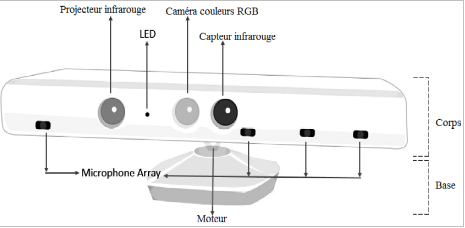
\includegraphics[scale=0.7]{images/fonctionnementdepth3d.png}
		\caption{Schéma illustratif des composants de la Kinect \textcolor[rgb]{1.00,0.00,0.00}{[11]} }
		\label{fig14}
	\end{figure}
	
	\subsubsection{Une caméra RGB (Red Green Blue)}
	Elle permet une prise d'image avec une fréquence de 30Hz, en couleur 32bits et en résolution VGA de 640x480 pixels. La caméra couleur est l'une des premières embarquées dans la technologie Kinect. Cette caméra contient essentiellement un capteur photographique de type CMOS.
	
	\subsubsection{Un capteur de profondeur}
	La technologie de la Kinect se voit dans son "Capteur de profondeur 3D", une technologie proposée pas la société PrimeSense. On retrouve à droite une caméra infrarouge à capteur CMOS, QVGA de résolution 320x240, et à gauche un émetteur de lumière infrarouge (voir figure \ref{fig1e5}).
	
	\begin{figure}[H]
		\centering
		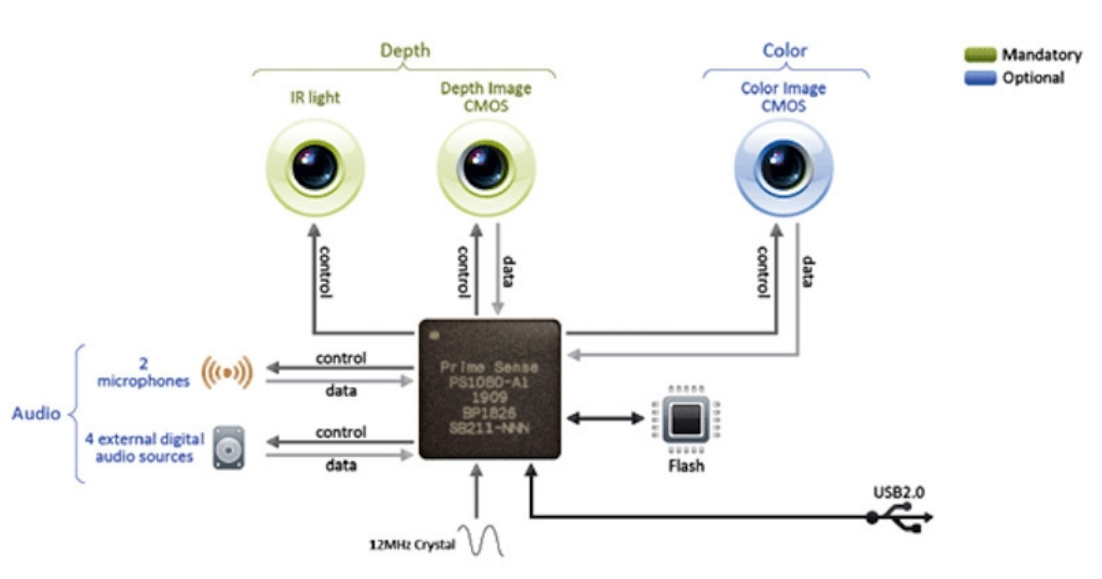
\includegraphics[scale=0.4]{images/composantkinect.png}
		\caption{Schéma explicatif du fonctionnement du capteur de profondeur \textcolor[rgb]{1.00,0.00,0.00}{[11]} }
		\label{fig1e5}
	\end{figure}
	
	
	Contrairement à la caméra RGB, dans ce cas on laisse passer uniquement les infrarouges, c'est à dire que les images obtenues ne sont pas colorées. La caméra infrarouge permet d'obtenir une image représentant les dégagements thermiques émis par l'objet observé.
	
	On détermine la distance d'un objet par rapport à la Kinect grâce a l'émetteur de lumière infrarouge, plus l'objet sera proche et plus la quantité de rayonnement infrarouge réfléchie sera importante et inversement plus il sera loin plus cette quantité sera faible. Il faut aussi préciser que les joueurs doivent être à une distance supérieur à $1.5-2$ mètres de la caméra et inférieur à $4-5$ mètres pour être bien détectés .
	
	On constate donc quelques avantages de l'utilisation de l'infrarouge [12]:
	\begin{itemize}
		\item La détection se fait dans toutes les conditions de luminosité.
		\item La charge du calcul de la machine est allégée car les cartes de  profondeur sont déjà calculées(30/seconde).
		\item Cette lumière est aussi insensible aux bruits et aux vibrations.
	\end{itemize}
	En revanche, l'infrarouge est limité car:
	\begin{itemize}
		\item Il est sensible aux variations de températures.
		\item Sensible au courant d'air.
		\item Sensible au soleil (forte source de lumière).
		\item La portée est limitée.
		\item La résolution de la carte de profondeur est de 640 x 480 pixels, la précision de la Kinect est d’environ 1 cm (ce qui pose problème  pour les petites surfaces).
	\end{itemize}
	
	\subsubsection{Un microphone}
	Ce microphone multi-array, contient quatre microphones qui sont situés le long du bord inférieur avant du capteur Kinect. Utilisés essentiellement pour la reconnaissance vocale, enregistrement de l'audio et pour trouver l'emplacement de la source sonore et la direction de l'onde audio.
	
	\subsubsection{Une base motorisée}
	Un entraînement mécanique situé dans le support du capteur Kinect incline automatiquement la tête du capteur vers le haut et vers le bas si nécessaire.
	
	\subsubsection{Light Emiting Diod}
	Placée entre la caméra et le projecteur infrarouge, il est utilisé pour indiquer l'état du dispositif Kinect. Il peut prendre 3 couleurs (rouge, jaune et vert), par exemple la couleur verte du LED indique que les pilotes des périphériques Kinect ont été chargés correctement.
	
	\subsection{Exemples d'application du capteur KINECT}
	Non destinée initialement à une commercialisation grand public, le produit Kinect, grâce a ses caméras de profondeur, a ouvert un immense champ d’applications dans certains domaines bien spécifiques.
	
	Dans l’industrie: Sonny par exemple a équipé une chaine de ces téléviseurs de capteur, pour remplacer la télécommande. L'industrie automobile l'utilise aussi afin d’augmenter la sécurité de déplacement des véhicules.
	L'industrie de la mode s'en sert aussi, à titre d'exemple,  en Russie la chaîne de vêtements Topshop a équipé ses magasins de Kinect pour habiller virtuellement ses clients.
	
	Dans le domaine paramédical et médical: le capteur est utilisé pour la pratique de la kiné à domicile, grâce a un programme qui permet aux patients de suivre leurs mouvements et les alerter s'ils n'ont pas la bonne technique.
	
	Parmi les projets ayant utilisé la Kinect, citons:
	
	\subsubsection{Dessin en air}
	Le dessin dans l'air est une application qui consiste à pouvoir dessiner ou écrire face à une caméra de profondeur sur une surface aérienne, le dessin résultant sera transcrit sur une image numérique ou projeté sur un mur avec un data show. Cette discipline exploite des données de profondeur sur un système de vision tridimensionnelle.
	
	L'approche choisie pour la réalisation d'une surface aérienne , est le calibrage de la dimension de cette dernière ainsi qu'une détection d'objet tel que le stylo ou une main servant à émuler le vrai outil d'écriture [8].
	
	\begin{figure}[H]
		\centering
		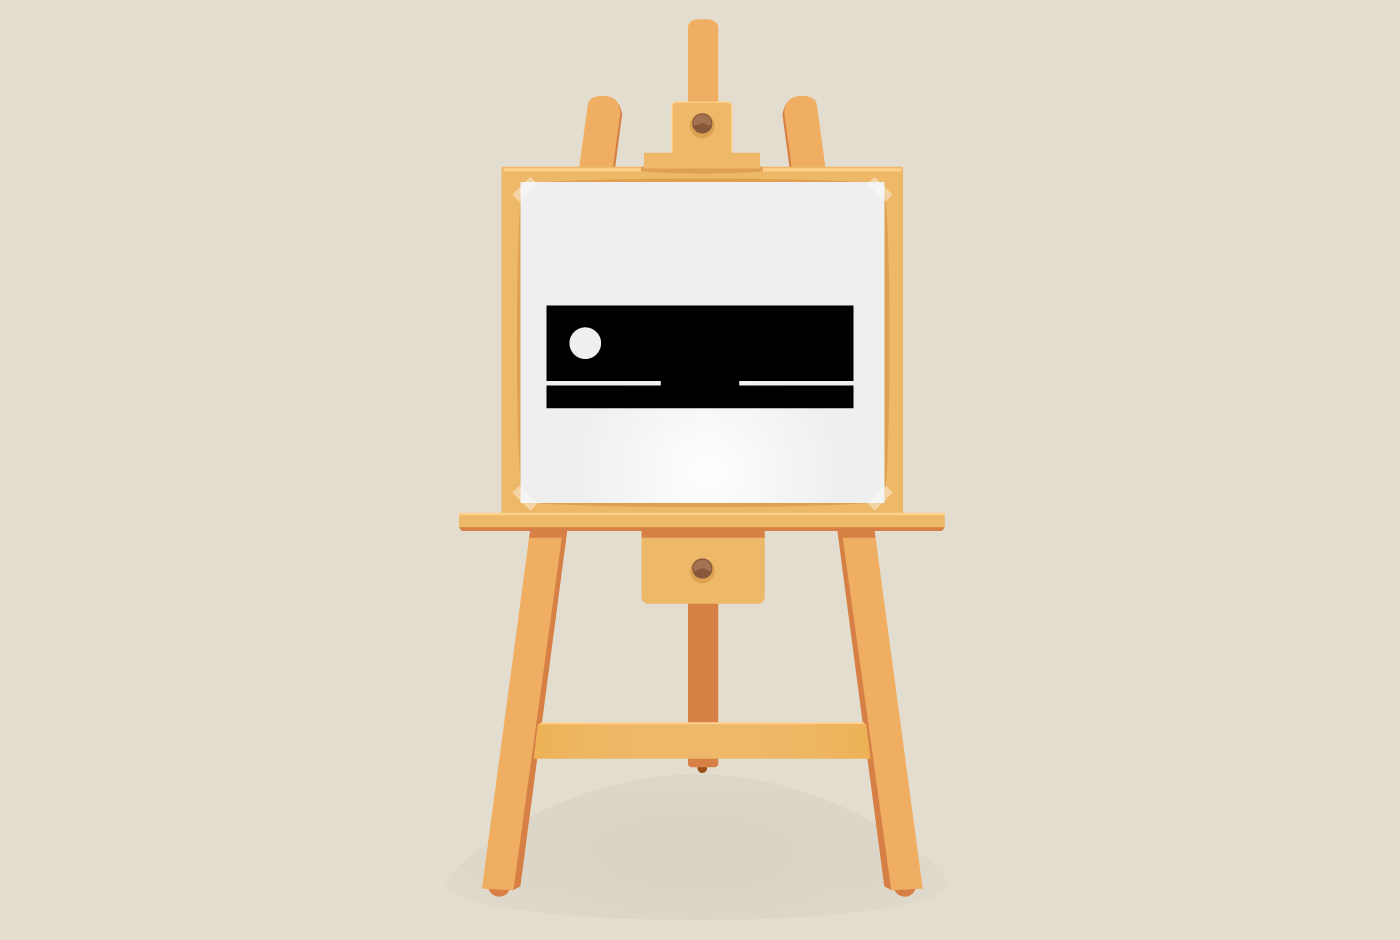
\includegraphics[scale=0.30]{images/kinect-drawing.png}
		\caption{Émulateur d'un tableau de face \textcolor[rgb]{1.00,0.00,0.00}{[8]}}
		\label{fig}
	\end{figure}
	
	
	\subsubsection{Le Mur Tactile}
	C'est un projet développé sous la direction de S. Larabi [9], il consiste à développer une solution permettant de rendre n’importe quelle surface plane, lisse, et unie, en une surface tactile équivalente à un écran tactile géant. Ainsi l’interaction avec cette surface sera au touché et ne nécessitera ni souris, ni clavier, ou tablette mais simplement un contact avec la surface de projection (un mur par exemple). Ceci se fait en délimitant la zone de traitement et en détectant les objets qui interagissant avec l'écran à l’intérieur de la zone. Ainsi qu'avec un système d’information assurant la communication entre les acteurs interagissant avec le mur \cite{9} (voir figure \ref{figm}).
	
	En ce qui concerne la détection d'objet, qui est très importante pour ce projet, on doit passer par plusieurs étapes:
	\begin{itemize}
		\item Parcours de la zone de traitement colonne par colonne (horizontalement de gauche à droite).
		\item Récupération de deux tableaux de profondeur (un pour la colonne courante et un pour la suivante).
		\item Validation, garder l'index du premier, avancer.
		\item Création d'objet si au minimum deux tableaux sont successivement validés entre eux.
		\item Délimitation des bordures de l'objet (validation des tableaux récupérées lors du parcours).
		\item Calcul de la profondeur moyenne pour chaque tableau.
		\item Comparaison avec chaque case du tableau, un tableau est dit valide si toutes les valeurs sont incluses dans un intervalle proche de la moyenne.
		\item Instanciation. Une fois l'objet détecté on crée une instance de la classe DetectedObject ou on sauvegarde : la position de l'objet(l'indice de la première colonne valide et celui de la dernière), la valeur de profondeur au milieu centre, milieu gauche, milieu droit. La longueur réelle de l’objet est calculée automatiquement.Ces informations seront utilisées par la suite dans d'autres traitements.
		\item Calcul des coordonnées (x, y) réelles de l'objet grâce au calibrage.
		\item Traduction de la détection d'objet en un événement clique comme la souris.
	\end{itemize}
	
	\begin{figure}[H]
		\centering
		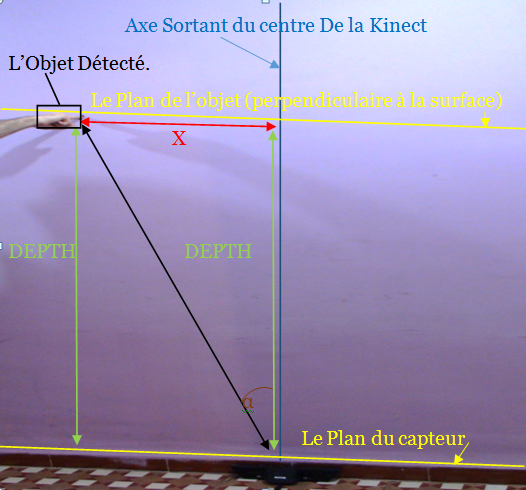
\includegraphics[scale=0.62]{images/m1.png}
		\caption{Le mur tactile}
		\label{figm}
	\end{figure}
	
	
	
	\subsubsection{Estimation de la direction du regard grâce a la Kinect}
	
	C'est un projet réalisé sous la direction de S. Larabi \cite{10} qui consiste à proposer une méthode pour l’estimation du regard, en exploitant le capteur Kinect. Cette méthode se base sur l'extraction de l'orientation du regard à partir de la pose de la tête, puis l'étude des différentes rotations de cette dernière.
	Les régions du visage sont exprimées en profondeurs, et la symétrie bilatérale et la partie du visage la plus proche du capteur. En positionnant le capteur de la Kinect droit par rapport à la tête de la personne, on peut estimer la direction du regard en temps réel à partir de sa pose des trois degrés de liberté de la tête: l’inclinaison par rapport au corps (Roll), l’inclinaison horizontale (Pan) et l’inclinaison verticale (Tilt)[10] (voir figure \ref{fig1f}).
	
	La méthode proposée s'exécute en deux étapes :
	\begin{itemize}
		\item La première étape est la récupération des données de profondeurs depuis le capteur Kinect puis la construction de la carte de profondeur du visage à partir de ces données.
		\item La seconde étape est l’extraction des caractéristiques nécessaires de la carte de profondeur du visage afin d’estimer la direction du regard correspondante à chaque pose.
	\end{itemize}
	
	\begin{figure}[H]
		\centering
		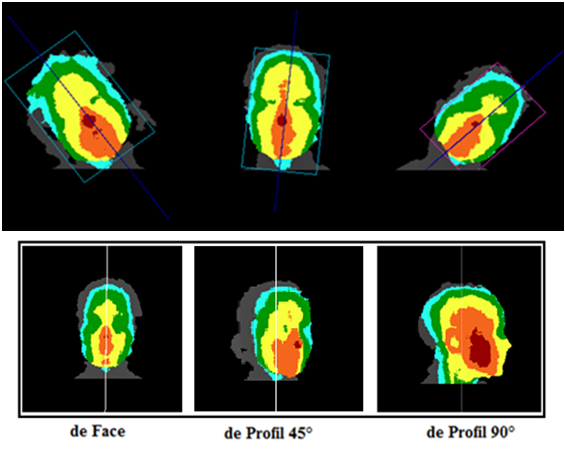
\includegraphics[scale=0.6]{images/v1.png}
		\caption{ Mouvement du visage }
		\label{fig1f}
	\end{figure}
	
	
	
	\section{Conclusion}
	Dans ce chapitre on a introduit les différents concepts liés au domaine de la vision artificielle, tels que les différents systèmes de vision artificielle et la reconnaissance d'objets.
	Ensuite, on a présenté la technologie Kinect qui sera exploité par la suite dans la conception de notre application.
	Enfin, on a cité quelques exemples d'application du capteur Kinect dans le domaine de la vision artificielle.
	
	Dans le chapitre suivant, on présentera le travail de conception de l'émulation d'un tableau moyennant la Kinect.
	
	
	
	
	
	
	\chapter{Conception}
	
	\section{Introduction}
	
	Dans ce chapitre on abordera en détails les différentes étapes menées afin de réaliser et développer le projet  ainsi que les approches choisies dans le but d'optimiser et améliorer ce dernier. Le schéma de la figure \ref{fig1a} résume les étapes de notre approche.
	
	
		\begin{figure}[H]
			\begin{center}
			\scalebox{1.2}{	\smartdiagram[priority descriptive diagram]{
					Détecter l'objet le plus proche,
					Calibrage du tableau,
					Détection d'écriture,
					Calcul de coordonnées réelles,
					Transcription vers un écran
				}}
				
			\end{center}
			\captionof{figure}{Schema explicatif du déroulement de l'application}
			\label{fig1a}
		\end{figure}
	La conception de notre application nécessite de suivre un certain processus , qui se résume avec  les points suivant :
	
	\section{Récupération du flux de données de la KINECT}
	
	Comme cité dans le chapitre précédent, le capteur 3D est doté d'une technologie permettant d'acquérir des informations de profondeur. Ainsi, il nous faudra en premier lieu:
	
	\subsection{Initialisation}
	En utilisant les fonctions du "developer toolkit", la Kinect est initialisée en mettant les flags qui permettent de récupérer le flux de données voulu qui peut être affiché comme pour n’importe quelle caméra.
	
	Le capteur Kinect peut retourner le flux en 640x480 (à 30 images par seconde) et en 1280x960 (mais à 15 images par seconde) pour l'image rgb. Le flux de profondeur est le facteur déterminant. 
	
	Il va, en effet, donner à chaque pixel une profondeur depuis le capteur. Ainsi en plus de la position en 2D de chaque pixel(ligne ,colonne) dans l'image profondeur, on dispose de leurs profondeurs (distance).
	
	
	\subsection{Traitement }
	Pour pouvoir récupérer la distance, on utilise le fait que le capteur sauvegarde dans chaque pixel qui est représenté sur 16 bits, la distance des objets sur 13 bits de poids forts ainsi que l'indice de joueur reconnu sur 3bits ce qui permettra de reconnaitre 8 joueurs.
	
	Ceci n'étant pas l'unique manière de procéder car on peut quand même, grâce à un autre flag qu'on passe en paramètre dans une fonction de la bibliothèque Kinect, réduire le nombre de joueurs trackés ( reconnus), il sera sur 2bits (ce qui veut dire qu'on reconnait maximum 4 joueurs), la distance qui sera sur 14bits, une distance max reconnue de $2^{14}-1$ mm.
	
	Afin de pouvoir manipuler cette distance, il suffit de faire un décalage à droite pour avoir ce flux (voir figure \ref{fig1d}).
	
	\begin{figure}[H]
		\centering
		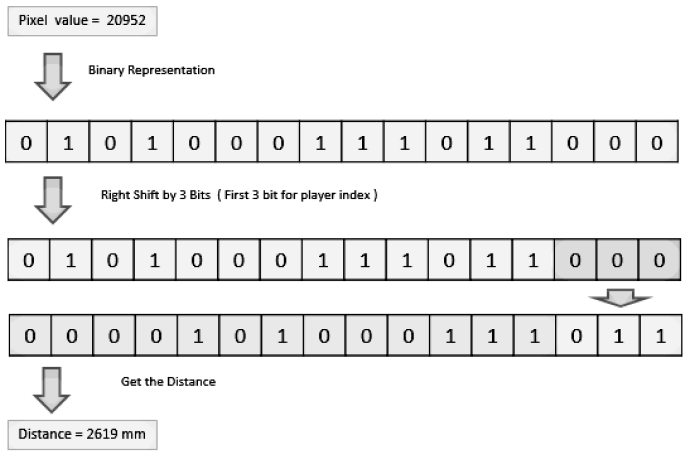
\includegraphics[scale=0.6]{images/screenshot001.png}
		\caption{Illustration du décalage \textcolor[rgb]{1.00,0.00,0.00}{[13]}}
		\label{fig1d}
	\end{figure}
	
	\subsection{Affichage relatif à la profondeur}
	
	Par définition une image de profondeurs est une matrice d'une dimension particulière où chaque case (pixel) identifiée par (ligne,colonne) est portante  d'une information profondeur et un indice joueur qui s'étale sur 16bits.
	En pratique, pour représenter une image en fonction des distances des pixels par rapport au capteur de profondeur Kinect, il faut attribuer une nuance de gris relative à cette dernière, plus précisément on va transformer les informations concernant la profondeur codée sur 13 bits en une intensité de gris codée sur 8bits.
	
	Les parties les plus claires indiqueront les objets proches, les plus sombres en revanche refléteront les objets les plus lointains, ainsi on peut afficher une couleur représentative de la profondeur. Un exemple est illustré par la figure \ref{fig1i}.
	
	\section{Détection de l'outil d'écriture}
	En pratique, la reconnaissance d'objet ou le tracking avec la technologie Kinect, se fait avec une multitude de méthodes et d'analyses de l'image profondeur.
	
	Nous allons procéder de telle sorte que l'objet le plus proche de la Kinect soit l'outil d'écriture.
	Notre méthode consiste à récupérer de la matrice ou la trame, la profondeur la plus petite,  une fois  trouvée , on va sauvegarder les coordonnées (ligne colonne de ce pixel).
	
	On doit ensuite faire en sorte que ce pixel ainsi que les pixels de l'outil d'écriture soient visibles, on a donc choisi de donner une couleur à ce pixel ainsi qu'aux pixels voisins car l'outil a une certaine épaisseur, par conséquent pour le rendre visible il faut cibler tous les pixels qui le représentent.
	
	Il s'agit ensuite de donner une couleur en rgb (red, green, blue) pour l'ensemble des pixels de la zone localisée (voir figures \ref{fig1i}, \ref{fig1c}).
	
	\begin{figure}[H]
		\centering
		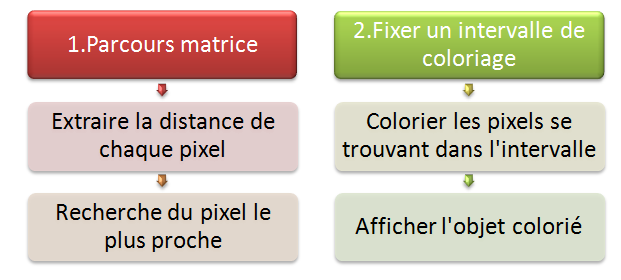
\includegraphics[scale=0.75]{images/s2.png}
		
		\captionof{figure}{Schéma explicatif de  la détection d'ojbet }
		\label{fig}
	\end{figure}
	
	\begin{figure}[H]
		\centering
		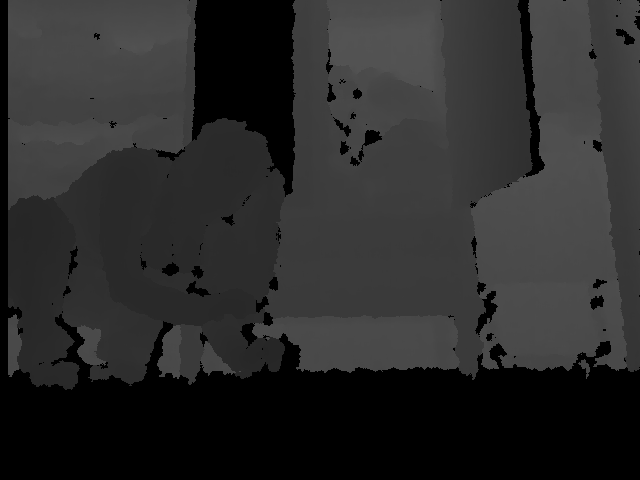
\includegraphics[scale=0.5]{images/image2.png}
		\caption{Image profondeur monochrome}
		\label{fig1i}
	\end{figure}
	
	\begin{figure}[H]
		\centering
		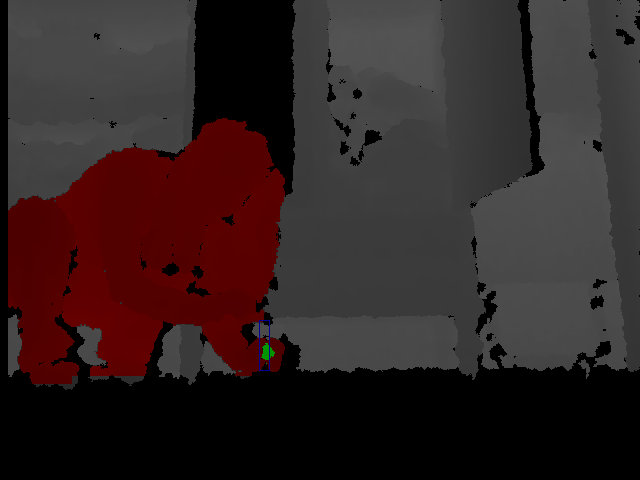
\includegraphics[scale=0.5]{images/hassinapixelrouge3.png}
		\caption{Image profondeur avec Coloriage d'un objet}
		\label{fig1c}
	\end{figure}
	
	\begin{figure}[H]
		\centering
		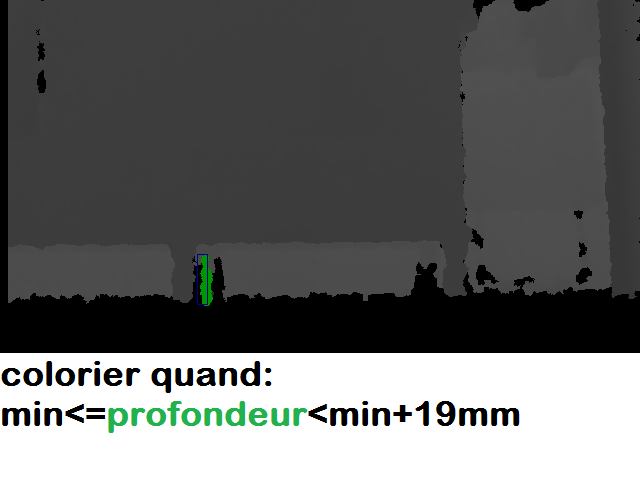
\includegraphics[scale=0.5]{images/i5.png}
		\caption{L'intervalle choisi pour le coloriage de l'outil}
		\label{figd0}
	\end{figure}
	
	\section{Calibrage du support d'écriture}	
	Sachant que le but de notre  application est d'écrire sur un support ayant  des dimensions fixes et connues puis aboutir à une écriture  parallèle sur l'écran d'un ordinateur de façon à faire en sorte que les deux écritures soient similaires et momentanées, on se confronte alors à une problématique qui réside dans l'interprétation des coordonnées $(x,y)$ dans le vrai support d'écriture et leurs translations  dans une fenêtre (image numérique simulant un tableau)  de dimensions connues.
	
	On peut résumer le processus de Calibrage \& le calcul de coordonnées par le schéma suivant (voir figure \ref{fig1s}).
	
	\begin{figure}[H]
		
			\begin{center}
				\smartdiagramset{
					uniform color list=blue!60!white for 8 items,
					back arrow disabled=true,
					module minimum width=2cm,
					module minimum height=2cm,
					module x sep=4cm,
					text width=3cm,
					additions={
						additional item offset=20mm,
						additional item width=2cm,
						additional item height=2cm,
						additional item text width=3cm,
						additional item shadow=drop shadow,
						additional item bottom color=red!30!white,
						additional item border color=gray,
						additional arrow color=red!66!white,
					}}
					\smartdiagramadd[flow diagram:horizontal]{
						Introduire la largeur et la hauteur,Délimitation de la zone d'ecriture, Déduction de la hauteur via profondeur,
						Extraire le pixel de largeur max
					}{
					below of module1/	Extraire le pixel de largeur 0 cm,below of module2/Calibrage,below of module3/Calcul du déplacement en largeur,below of module4/Calcul du déplacement en hauteur
				}
				\smartdiagramconnect{->}
				{additional-module1/additional-module2,additional-module2/additional-module3,
					additional-module3/additional-module4}
				\begin{tikzpicture}[remember picture,overlay]% modified from p. 47 of manual
				\draw[additional item arrow type] (module4) |- ([yshift=-10mm]module1.south) -- (additional-module1);
				\end{tikzpicture}
				\vspace{40mm}\par
				
			\end{center}
		\captionof{figure}{Processus résumant le Calibrage du support et calcul des coordonnées réelles}
		\label{fig1s}
	\end{figure}

	\subsection{Émulation de l'écriture}
	
	Les limites d'une zone rectangulaire servant comme support d'écriture ayant des profondeurs différentes et connues servent à localiser la profondeur de tout pixel entre les deux limites. Un exemple est illustré dans la figure \ref{fig1m}.
	On  remarque facilement que la largeur de la limite proche est supérieure à la largeur de la limite lointaine.
	Ceci nous amène à procéder à son calibrage qui consiste à déterminer la relation mathématique existante entre les coordonnées des points de la scène d'écriture et les coordonnées 2D de leur projection dans l'image.
	
	\begin{figure}[H]
		\centering
		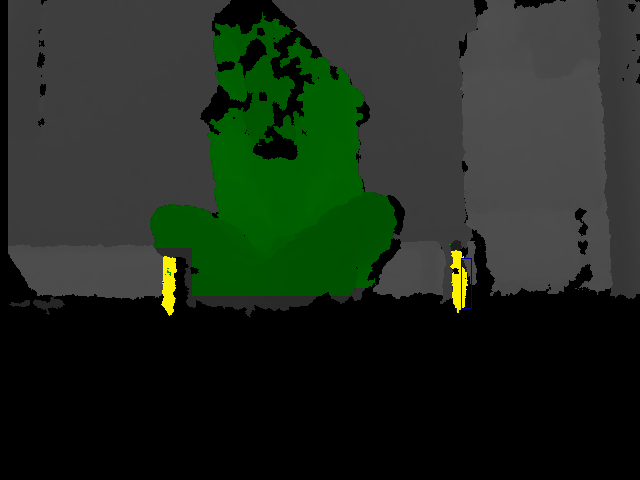
\includegraphics[scale=0.45]{images/simuler.png}
		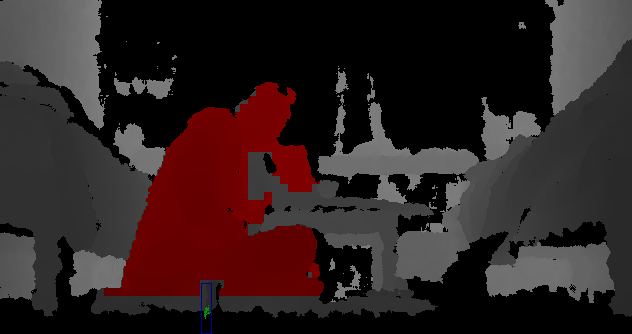
\includegraphics[scale=0.45]{images/i6.png}
		\caption{Image de profondeurs à 1000mm (à gauche) et à 1470mm (à droite) pour une zone de 50cm}
		\label{fig1m}
	\end{figure}
	
	Le calibrage se fait comme suit:
	
	\begin{figure}[H]
		\centering
		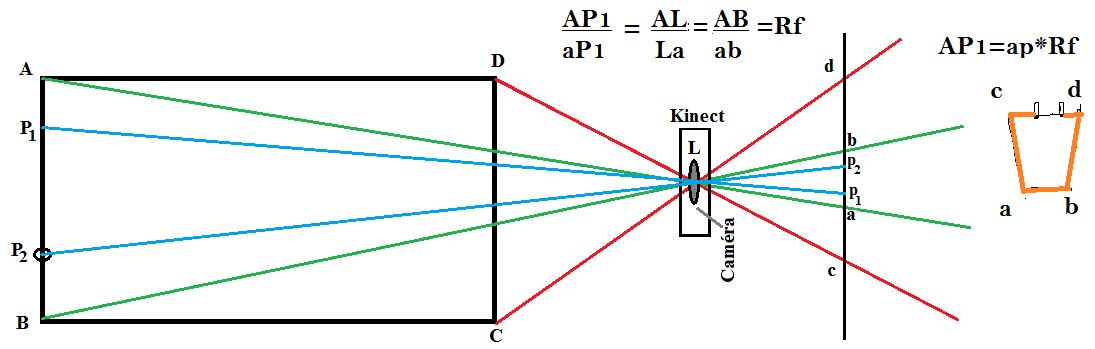
\includegraphics[height=9cm ,width=15cm]{images/imn1.png}
		\caption{Déplacement en lignes sur le tableau}
		\label{fig1nn}
	\end{figure}
	
	D'après la figure \ref{fig1nn}, si $AB$ et $CD$ se projettent en $ab$, $cd$ et si le stylo $P$ en $3D$ se déplace le long de $AB$, sur l'image il se déplacera le long de la ligne $ab$, alors il est facile de démontrer que $P$ est localisé avec  la relation:
	$AP= ap \times r_f$ où $r_f=AB/ab$ et $p$ est la projection du stylo $P$ sur l'image.
	
	Pour un déplacement en profondeur du stylo, ses positions en 3D sont déduites directement de leur position sur la colonne (voir figure \ref{fig2nn}).
	
	\begin{figure}[H]
		\centering
		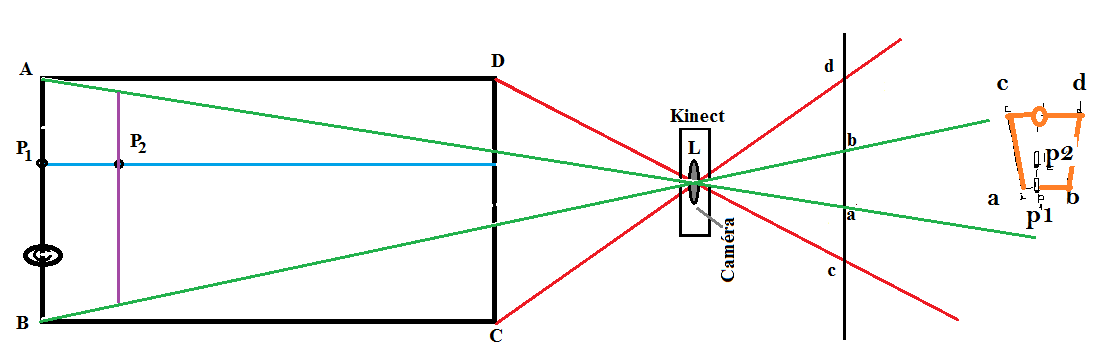
\includegraphics[height=7.5cm ,width=15cm]{images/imn2.png}
		\caption{Déplacement en lignes sur le tableau}
		\label{fig2nn}
	\end{figure}
	
	Donc pour récapituler on peut dire que la transcription de coordonnées se résume par les étapes suivantes illustrées par la figure 2.11.
	
	\begin{figure}[H]
		\centering
		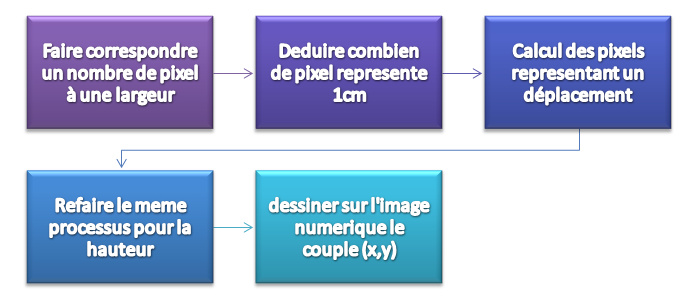
\includegraphics[scale=0.69]{images/s3.png}
		\captionof{figure}{Etapes essentielles pour la transcription de coordonnées}
		\label{fig100}
	\end{figure}
	
	
	\section{Précision de l'écriture: Où est la bille du stylo sur l'image de profondeurs}	
	
	Le problème posé consiste à trouver sur l'image de profondeurs le pixel correspondant à la bille du stylo se déplaçant sur la zone d'écriture.
	
	Or, en pratique, il n'est pas sûr que le(s) pixel(s) le(s) plus proche(s) dans l'image de profondeurs correspond(ent) à la bille.
	A titre d'exemple, si l'on considère le pixel le plus proche comme pixel correspondant à la bille, une ligne droite tracée par le style sera traduite vers des lignes avec zig-zag comme illustré par la figure \ref{figb}.
	
	\begin{figure}[H]		
		\centering
		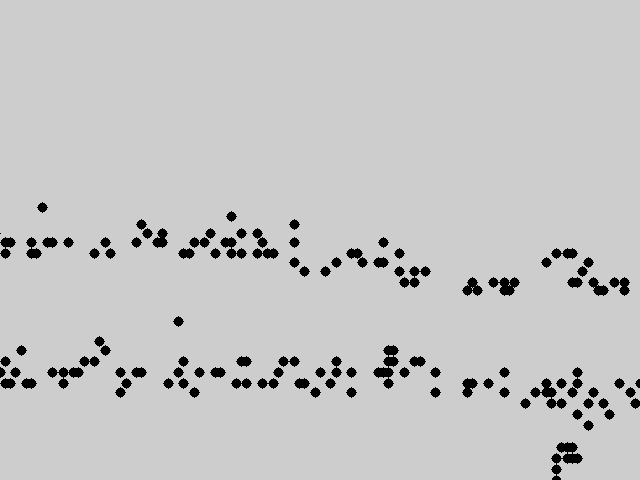
\includegraphics[scale=0.45]{images/A44.png}
		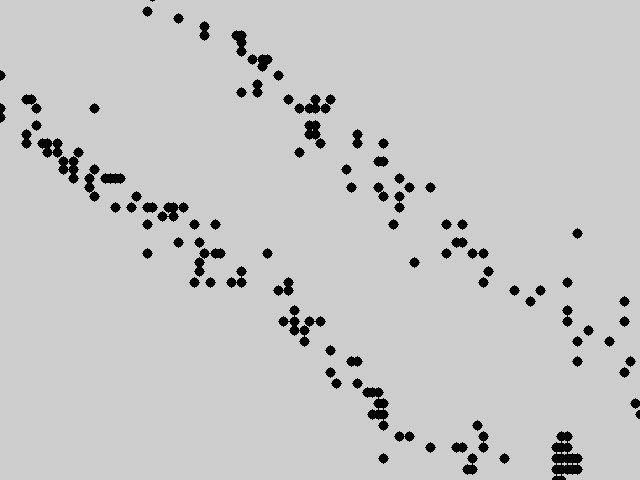
\includegraphics[scale=0.45]{images/FormatA41.png}
		\caption{Résultat du traçage de deux droites parallèle horizontales et inclinées}
		\label{figb}
	\end{figure}
	
	Il est important de préciser qu'on a effectué nos tests avec un seul calibrage qui est statique à distance fixe, non variable, pour des dessins réalisés dynamiquement sur un support d'écriture.
	
	
	\subsection{Amélioration de la détection de la bille}
	
	\subsubsection{Pixel plus bas}
	Dans le but de remédier au problème de détection de la bille ainsi que l'imprécision engendrée par ce dernier, on a mis en place une nouvelle approche qui consiste à trouver le pixel le plus bas parmi ceux  qui se trouvent dans l'intervalle de coloriage  pour que la position du pixel détecté soit la plus stable possible et non aléatoire, comme celle du plus proche.  Les résultats obtenues seront exposés dans le chapitre suivant.
	
	Les résultats avec le pixel le plus bas combiné ont donné une amélioration assez importante mais toujours loin de la perfection. On s'est alors  trouvé face à un nouveau problème de précision qui se présente en dessinant, dès qu'on s'arrête sur une position le programme continuer de dessiner des petites droites dans une zone minuscule faisant allusion que l'outil d'écriture bouge alors que ce n'était pas le cas, ceci reste principalement dû à la détection du pixel le plus bas cette fois-ci, le pixel reste quand même très mobile sur un flux  vidéo important traitant beaucoup de frames, et un mince changement de position l'affecte de façon amplifiée.
	
	\subsubsection{Pixel Barycentre}
	En géométrie, le barycentre est un point qui permet de résumer un ensemble géométrique sur lequel sont réparties des valeurs numériques [14].
	%	https://fr.wikipedia.org/wiki/Barycentre/_(géométrie_élémentaire).
	La prise en compte du barycentre de la zone la plus basse du stylo sur l'image de profondeurs a montré que cette approche est beaucoup plus stable sur un flux vidéo traitant toutes les frames,  car le barycentre a cette propriété de stabilité par rapport aux mouvements de la forme géométrique présentant notre outil d'écriture.
	
	\subsubsection{Nombre de frames}
	Comme ça été explicité dans le chapitre précédent, la Kinect fournit un flux vidéo de 30 frames par seconde avec une résolution de 640x480. Nous avons étudié dans les tests expérimentaux l'effet du changement du nombre de frames sur la qualité d'écriture. Les résultats obtenus sont donnés dans chapitre suivant.
	
	\subsubsection{Position moyenne sur un nombre de frames}
	Nous avons testé la prise en compte de la moyenne des positions de la bille sur un ensemble de frames au lieu d'une frame. 
	
	\section{Arrêt et effaçage de l'écriture}
	L'approche proposé se base sur le protocole suivant :
	
	\begin{itemize}
		\item 	On sauvegarde premièrement la ligne dans l'image  profondeur  de l'objet d'écriture quand il est en contact avec le support durant le processus de calibrage.
		\item  On élève le stylo du support et on localise la bille sur l'image de profondeurs, la différence de position est alors considérée comme désactivant l'écriture.		
	\end{itemize}
	
	Pour modéliser la gomme, on suppose que l'outil d'écriture ou de dessin peut se transformer en un outil gomme en détectant la zone la plus proche ayant une largeur supérieure à celle qui est localisée précédemment.
	
	\section{Conclusion}
	Dans ce Chapitre on a proposé une approche initiale qui consiste à émuler un tableau en calibrant un support d'écriture puis déplacer l'outil sur la zone d'écriture. Ceci a été possible en exploitant des données de profondeurs extraites de la Kinect xbox 360 grâce à son capteur profondeur. On a ensuite énuméré d'autre approches proposées dans le but d'améliorer l'écriture ou le dessin qui va  être projeter sur un mur grâce à un data-show de façon à émuler un vrai tableau. Dans le chapitre suivant on présentera en images les résultats obtenus pour chaque approche.
	
	
	
	
	\chapter{Expérimentation et Résultats}
	
	\section{Introduction}
	
	Dans ce chapitre, on va en premier lieu présenter la  configuration logicielle et matérielle utilisées pour notre projet. Ensuite on présentera un scénario d'exécution et les résultats obtenus par chaque approche citée dans le chapitre précédent. Le fonctionnement de l'application est aussi illustré à travers des images d'exécution .
	
	
	\section{Environnement de développement}
	
	\subsection{Configuration matérielle et logicielle}
	
	L'application développée a été implémentée sur une machine ayant les caractéristiques suivantes:
	
	\begin{itemize}
		\item Processeur: Intel(R) Core(TM) i5-3317U @ 1.70Hz 1.70 GHz.
		\item Système d'exploitation: Windows 7 64bits.
		\item RAM: 8Go.
		%	\item Capteur Kinect pour Xbox 360.
		%	\item Adaptateur USB Kinect.
	\end{itemize}
	
	On a utilisé pour l'implémentation le langage de programmation \textbf{C++}, sous l’environnement de développement\textbf{Visual Studio C++}.
	
	De plus on a eu besoin de \textbf{Open Cv} qui est une bibliothèque graphique libre, spécialisée dans le traitement d'images.
	
	Aussi on a utilisé une Kinect Xbox 360  v1 (version 1) et son \textbf{SDK version 1.8}, qui est un kit de développement officiel Microsoft qui prend en charge les fonctionnalités de cette dernière, y compris les images en couleurs, les images de profondeurs, l'entrée audio et les données squelettiques.
	Dans notre cas on a eu besoin d'une seule fonctionnalité celle  des images de profondeurs  pour la détermination de la distance entre un objet et la caméra du capteur profondeur.
	
	
	\section{Scénario d'exécution}
	
	Tout d'abord  pour le bon fonctionnement de notre projet, il ne doit pas y avoir d'obstacles lors du calibrage. En effet, ils pourraient être détectés comme objet le plus proche de la Kinect. La Kinect doit être placée à environs 1.20 m de notre surface à calibrer. Par la suite, le processus se déroule comme suit:
	
	\begin{itemize}
		\item Entrer la largeur de la surface.
		\item Entrer la hauteur de la surface.
		
		\item Mettre l'outil le plus proche de la  Kinect 
		\item Appuyer sur "r" pour Calibrer la largeur en première position \textbf{0} cm en mettant l'outil dessus.
		\item Appuyer sur "r" pour Calibrer la largeur en seconde position \textbf{Max} cm en mettant l'outil d'écriture dessus.
		\item Appuyer une nouvelle fois sur 'r' pour le calibrage de troisième point correspond à une largeur 0 cm et une hauteur Max cm.
		\item Appuyer encore une  fois sur 'r' pour le calibrage de quatrième  point correspond à une largeur \textbf{Max } cm et une hauteur \textbf{Max} cm.		
		\item Appuyer une dernière fois sur "r", afin de commencer l'écriture et la visualiser sur l'écran.
	\end{itemize}
	
	\begin{figure}[H]
		
		\centering
		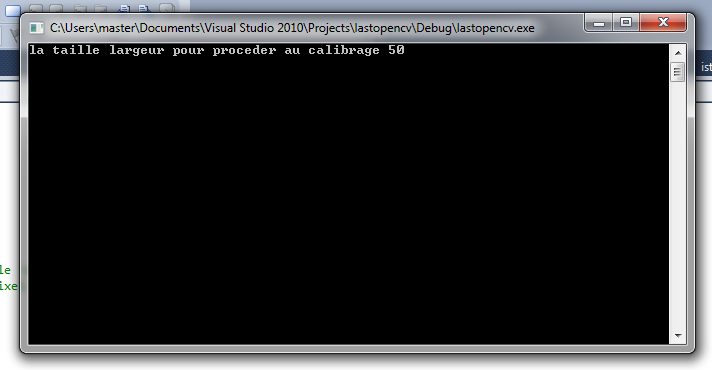
\includegraphics[scale=0.7]{images/it1.png}
		\caption{Introduction des dimensions du support}
		\label{fig8}
	\end{figure}
	
	\begin{figure}[H]	\centering
		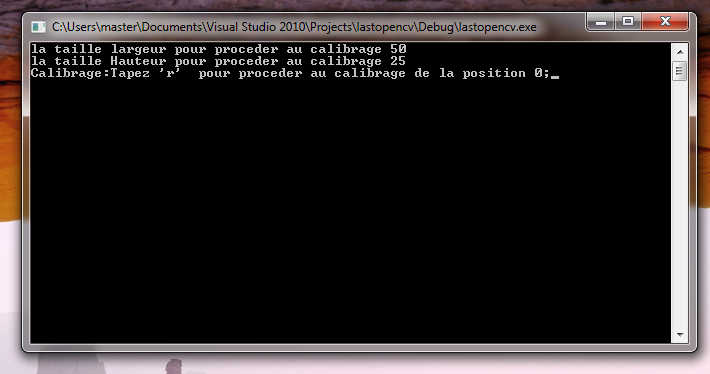
\includegraphics[scale=0.7]{images/it2.png}
		\caption{Introduction des dimensions du support}
		\label{fig9}
	\end{figure}
	
	\begin{figure}[H]
		\centering
		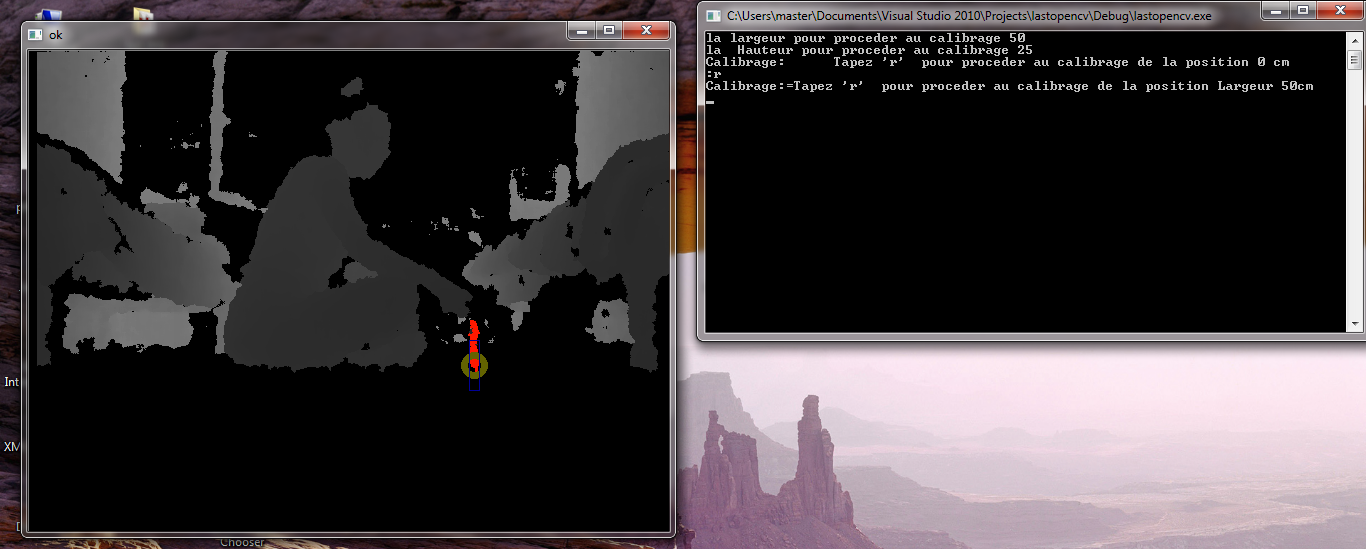
\includegraphics[scale=0.47]{images/it3.png}
		\caption{Calibrage du premier point}
		\label{fig10}
	\end{figure}
	
	\begin{figure}[H]
		\centering
		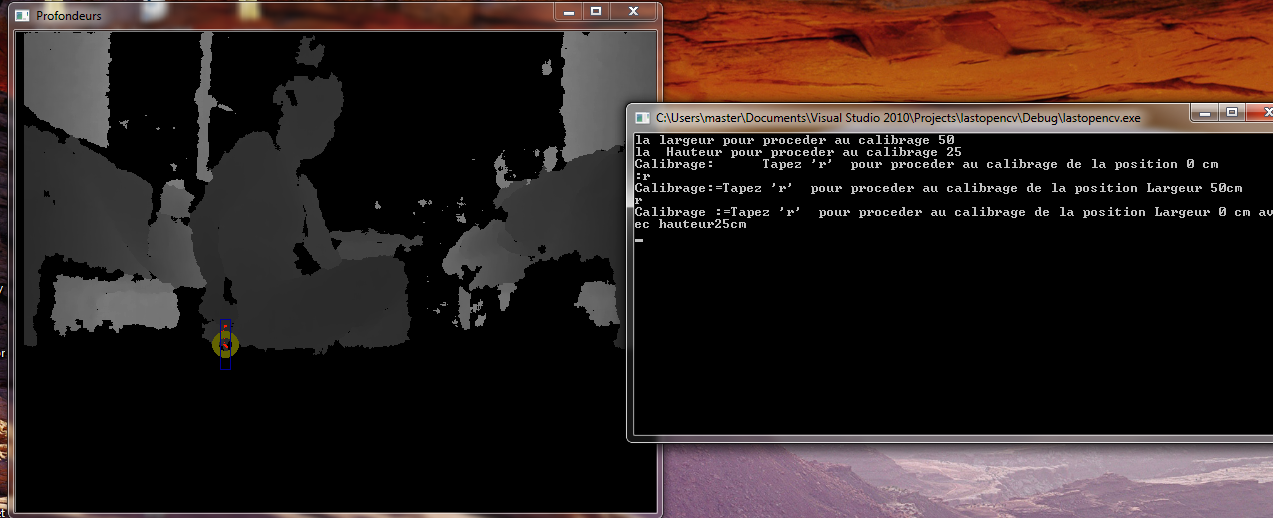
\includegraphics[scale=0.47]{images/it4.png}
		\caption{Calibrage du second point}
		\label{fig11}
	\end{figure}
	
	\begin{figure}[H]
		\centering
		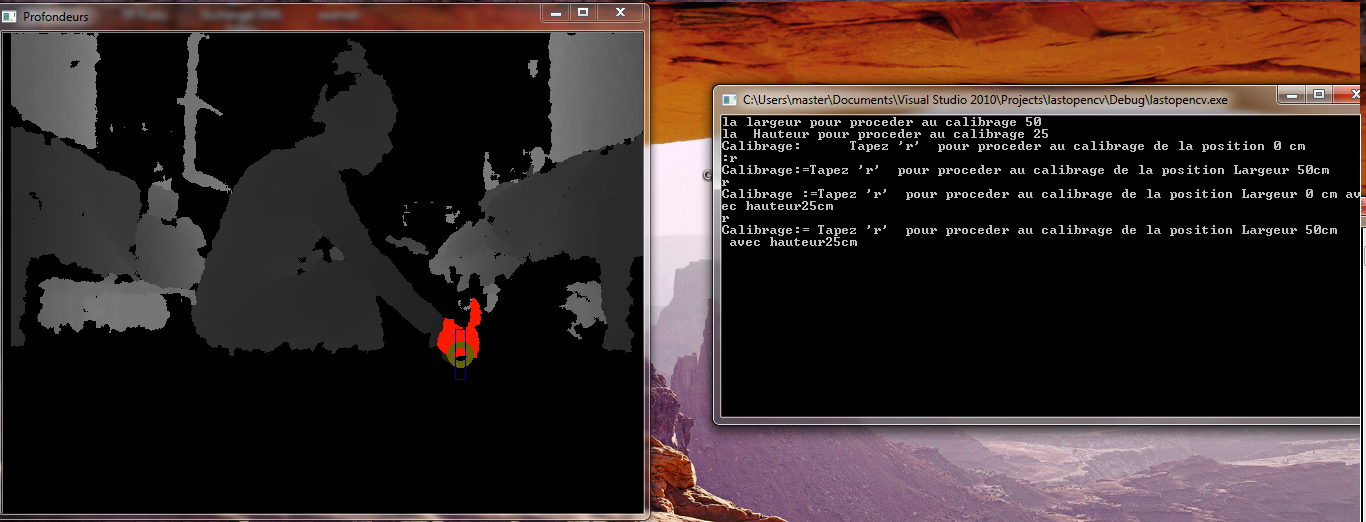
\includegraphics[scale=0.47]{images/it6.png}
		\caption{Calibrage du troisième point}
		\label{fig16}
		
	\end{figure}
	
	\begin{figure}[H]
		\centering
		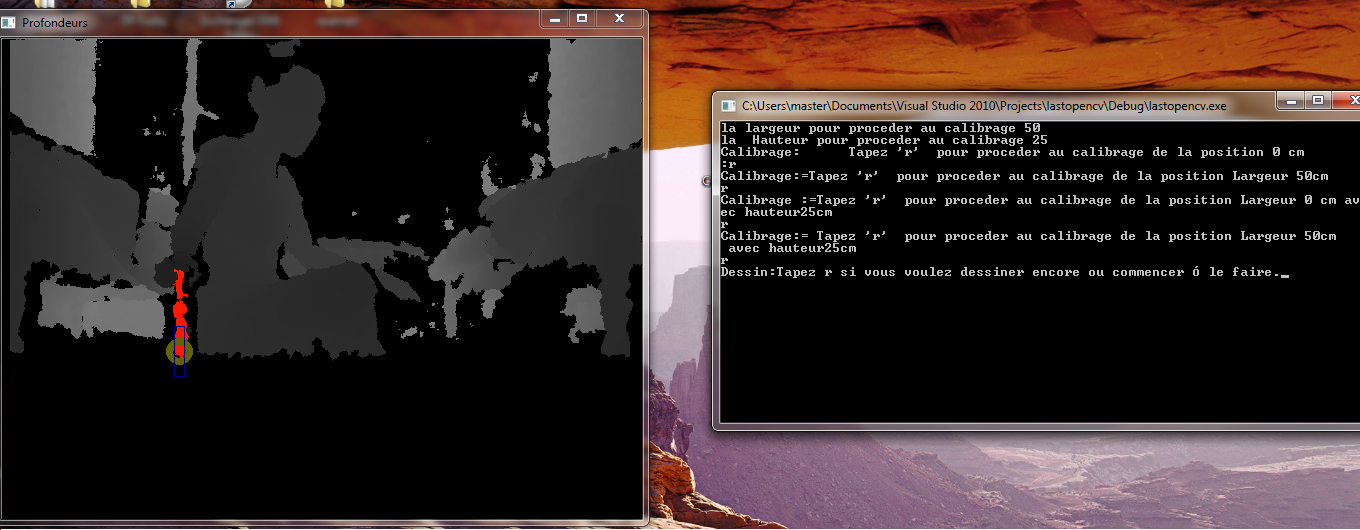
\includegraphics[scale=0.47]{images/it7.png}
		\caption{Calibrage du quatrième point}
		\label{fig17}
		
	\end{figure}
	
	
	\begin{figure}[H]
		\centering
		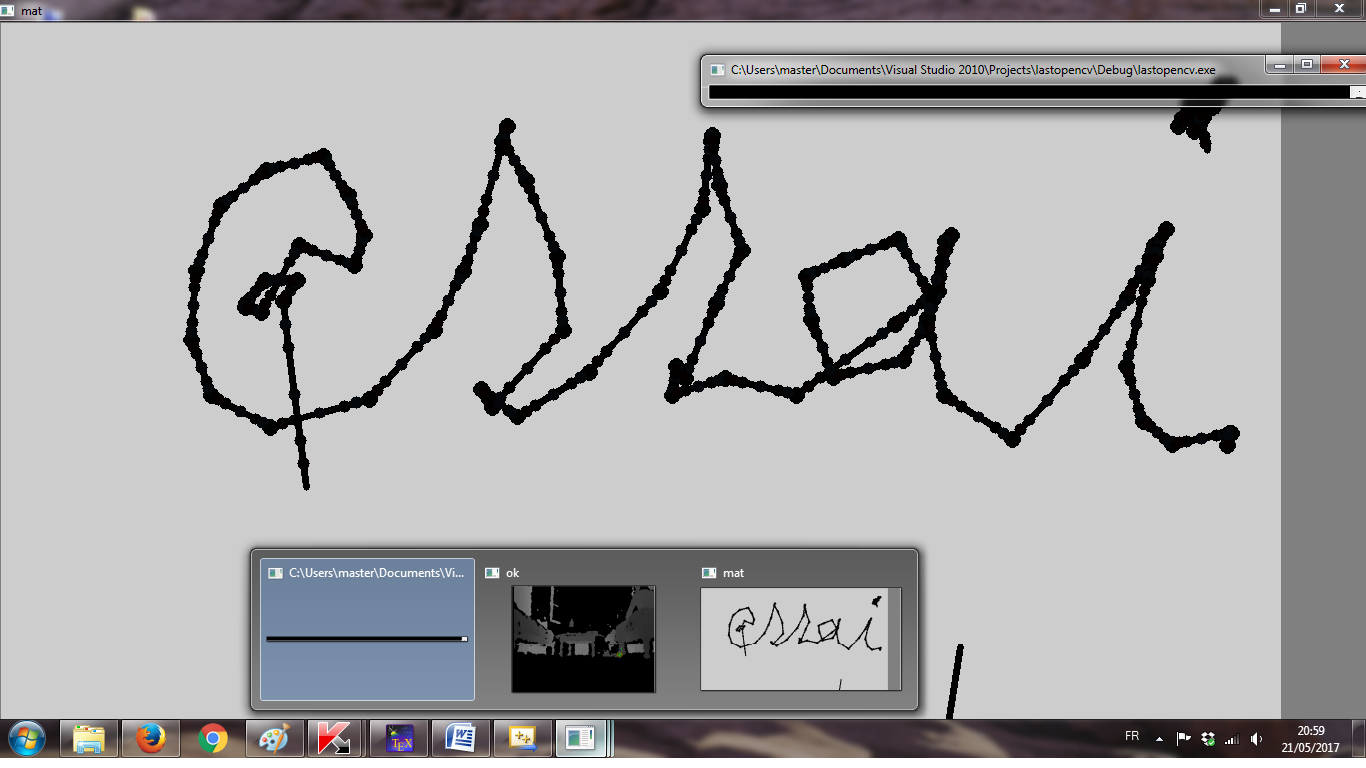
\includegraphics[scale=0.47]{images/it5.png}
		\caption{Début du dessin}
		\label{fig12}
		
	\end{figure}
	
	
	\section{Tests et résultats}
	
	La plateforme d'expérimentation se présente comme illustré par la figure \ref{fig15}. On voit une Kinect en face d'une zone d'écriture (tableau) avec un stylo pour écriture. Un ordinateur connecté à la Kinect, sur son écran est visualisée l'écriture.
	
	
	\begin{figure}[H]	
		\centering
		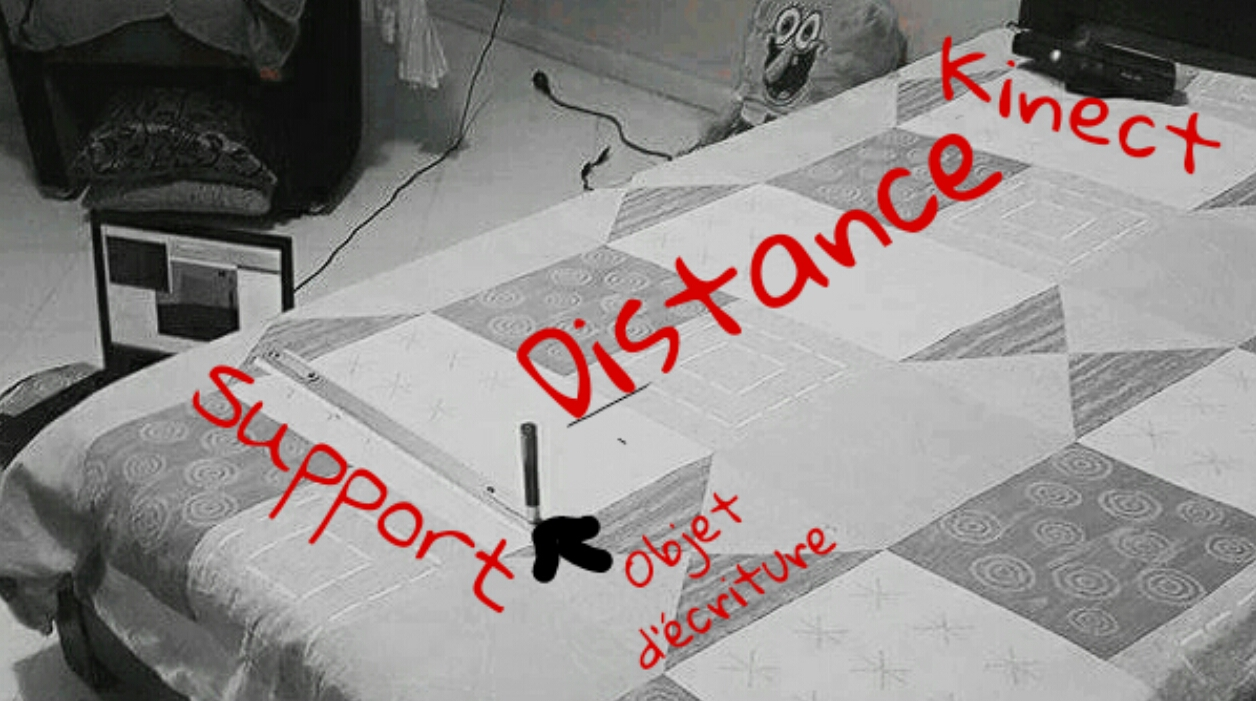
\includegraphics[scale=0.35]{images/exp.jpg}
		\caption{La Plateforme d'expérimentation}
		\label{fig15}
	\end{figure}
	
	
	Chaque approche proposée dans la conception sera illustrée par les figures suivantes.
	
	\subsection{Jointure des pixels "bille" par des segments de droites (avec le pixel le plus proche)}
	
	\begin{figure}[H]
		\begin{minipage}[H]{0.5\linewidth}
			\centering
			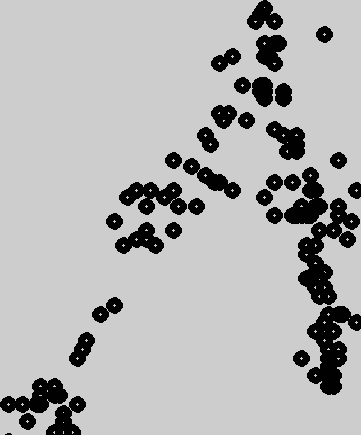
\includegraphics[scale=0.98]{images/avantp.jpg}
			\caption{Écriture sans utilisation \\des droites.}
			\label{fig19}
		\end{minipage}
		\begin{minipage}[H]{0.5\linewidth}
			\centering
			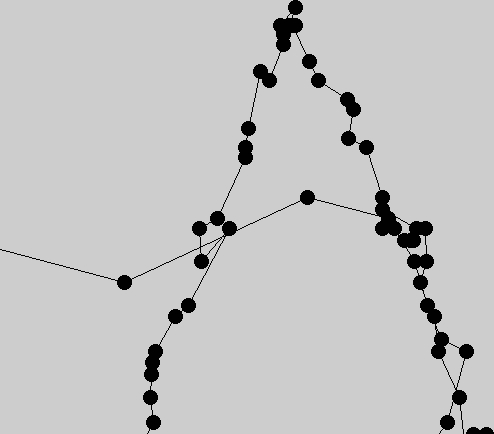
\includegraphics[scale=0.98]{images/apresp.jpg}
			\caption{Écriture avec utilisation \\des droites.}
			\label{fig20}
		\end{minipage}
	\end{figure}
	
	\subsection{Variation du nombres de frames}
	
	\begin{figure}[H]
		\begin{minipage}[H]{0.5\linewidth}
			\centering
			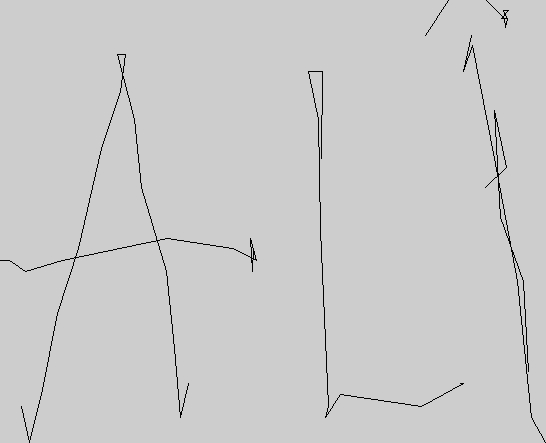
\includegraphics[scale=0.92]{images/12frame.jpg}
			\caption{Écriture avec 15 frames.}
			\label{fig1}
		\end{minipage}
		\begin{minipage}[H]{0.5\linewidth}
			\centering
			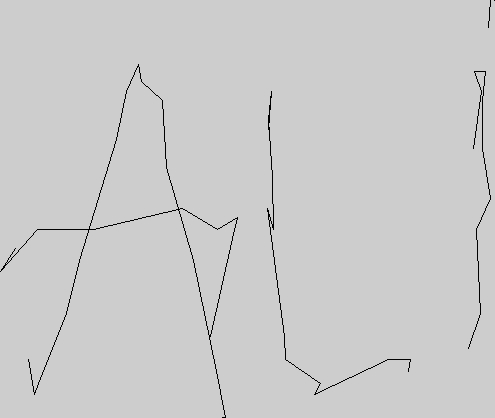
\includegraphics[scale=0.99]{images/8frame.jpg}
			\caption{Écriture avec 10 frames.}
		\end{minipage}
		
	\end{figure}
	
	\subsection{Considération du barycentre combiné à la moyenne de positions de la "bille" dans les frames}
	
	
	\begin{figure}[H]
		
		\centering
		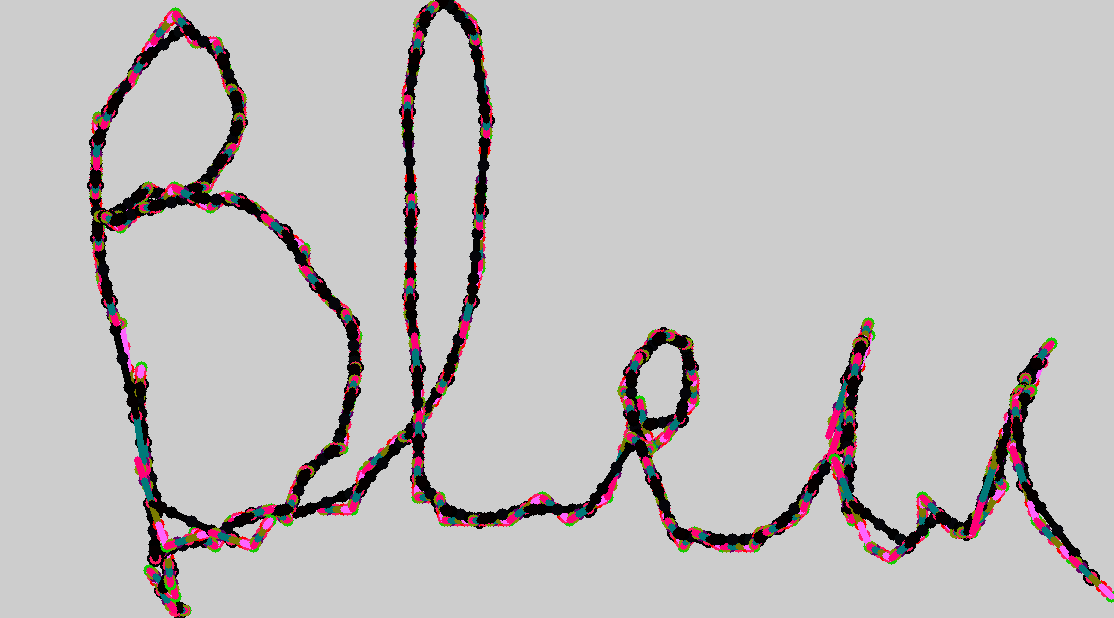
\includegraphics[scale=0.5]{images/bleubarycentremoyenne.png}
		\caption{écriture en noire avec moyenne des frames sur 15frames/secondes}
		\label{fig13}
		
	\end{figure}
	
	\begin{figure}[H]
		\centering
		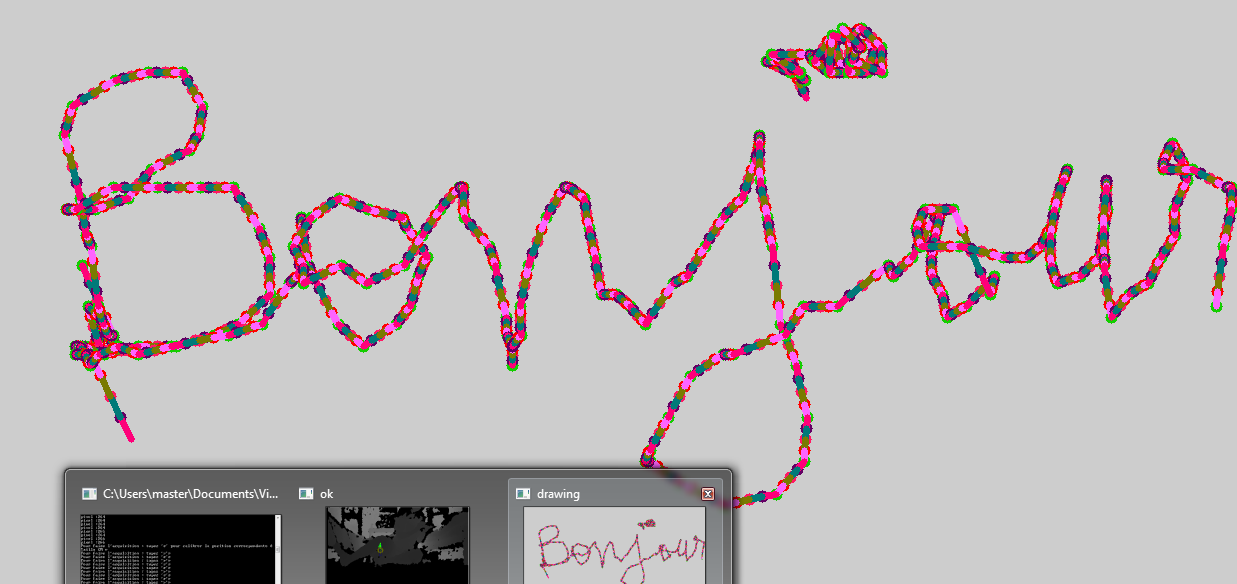
\includegraphics[scale=0.5]{images/bnjr.png}
		\caption{écriture coloré de 15frames/seconde}
		
	\end{figure}
	\section{Effaçage}
		\begin{figure}[H]
			\centering
			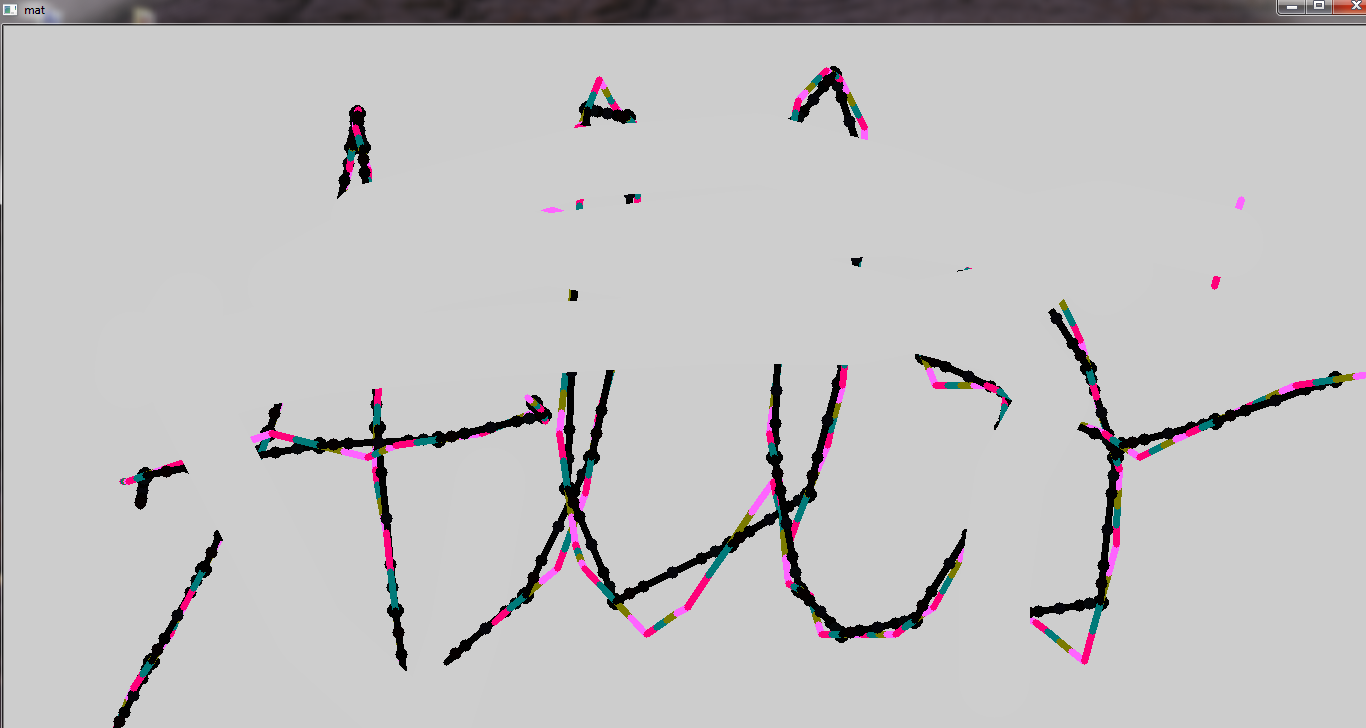
\includegraphics[scale=0.45]{images/ef1.png}
			\caption{ Application de l'option effaçage sur une écriture}
			
		\end{figure}
	
	\section{Discussion et travaux futurs}
	Après avoir travailler sur ce projet et compte tenu des résultats obtenus, il est clair que l'écriture ou le dessin qu'on peut exécuter sur un support d'écriture (tableau), reste toujours loin de l'écriture parfaitement intuitive ce qui peut être dû à une combinaison  de plusieurs taux d'erreurs au moment du calibrage ainsi qu'aux fonctions utilisées qui relient deux points par un segment, alors que l'écriture intuitive ressemble plus à des courbes.  
	
	Comme travaux futurs on peut penser à écrire une fonction qui reflète les courbes d'une écriture, de connecter notre programme à une base de données de l'alphabet latin ou arabe, pour l'exploiter lors de la reconnaissance de l'alphabet et correction de la forme de la lettre, qui éventuellement pourra être transformée l'écriture en script.
	
	Quant à l'option effacer, qui doit être enclencher par le simple fait d'utilisation d'un outil d'effaçage deux à trois fois plus largue que celui de l'écriture, on peut aussi le réaliser à l'aide d'une détection de la main face au capteur profondeur de la Kinect xbox 360. En d'autres termes, dés qu'on détecte une main on activera l'option effacer, ou bien on essayera de détecter une simple gomme avec des dimensions fixes introduites auparavant. Comme on a la possibilité de définir un protocole ou une action, tel que une position de la main ou bien de l'outil d'écriture face à la Kinect.%, grâce à laquelle on pourra effacer tel que lever l'index face à une kinect v2  par exemple qui offre beaucoup de possibilité.
	
	Notre projet peut être sujet à plusieurs autres propositions et idées qui contribueront à son amélioration.
	
	
	\section{Conclusion}	
	Dans ce chapitre on a illustré en images tous les résultats qu'on a obtenu pour chaque approche proposée dans le chapitre précédent dédié à la conception, dans le seul but d'améliorer l'écriture en la rendant plus lisible et la plus proche possible de l'écriture intuitive, on a explicité toutes les ressources, environnement de développement et le langage avec lequel on a implémenté notre programme. On a aussi illustré un scénario d'exécution représentatif du déroulement de notre application  puis on a listé les différents travaux futurs possible pour notre projet afin d'aboutir à un résultat proche plus satisfaisant. 
	
	
	\newpage
	\chapter*{Conclusion générale}
	\addcontentsline{toc}{chapter}{Conclusion générale}
	
	Ce mémoire avait pour objectif la proposition d'une méthode consistant à émuler un tableau moyennant une Kinect.
	
	Dans le premier chapitre on a définit tout ce qui est en relation avec le domaine de la vision artificielle.
	On a présenté quelques projets en relation avec la vision. 
	
	Nous avons ensuite expliqué, dans le second chapitre, les détails de conception étape par étape, puis on a proposé quelques approches pour de meilleurs résultats. 
	
	Pour finir dans le dernier chapitre  on a pu voir le processus  principal d'exécution de notre programme et montrer ainsi l'aboutissement des approches proposées.
	
	on est arrivés à un résultat où on peut détecter une écriture ou un dessin, grâce à n'importe quel outil d'écriture (stylo, feutre, doigt..), et  sur n'importe quel support  si  et seulement si les distances, pour une bonne détection, sont respectées. 
	
	Ce travail peut être  nettement améliorer par la suite pour avoir plus de précisions et un meilleur résultat. 
	
	
	
	%	\begin{figure}[!ht]
	%	\begin{minipage}[t]{7cm}
	%		\centering
	%		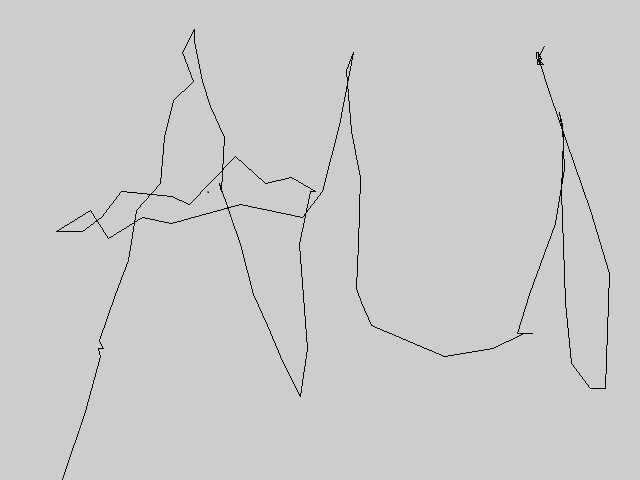
\includegraphics[scale=0.4]{ok5.png}
	%		\caption{écriture attachée}
	%		\label{fig1}
	%	\end{minipage}
	%	\begin{minipage}[t]{7cm}
	%		\centering
	%		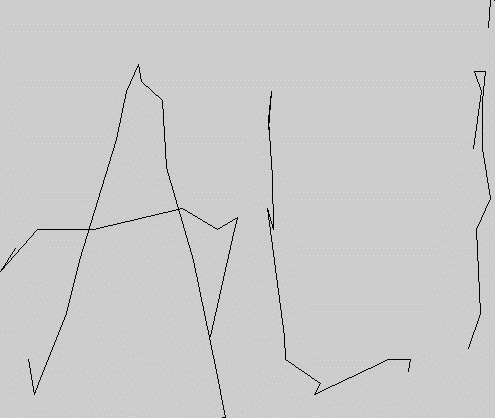
\includegraphics[scale=0.95]{ok.png}
	%		\caption{écriture détachée}
	%	\end{minipage}	
	%\end{figure}
	
	
	
	
	\newpage
	\pagenumbering{gobble}
	\begin{thebibliography}{20}
		
		\bibitem [1] {1} Définition de la vision par ordinateur. https://fr.wikipedia.org/wiki/Visionparordinateur.
		\bibitem[2] {2} N. Baha. Estimation de la carte de disparité en utilisant la méthode Neural-DSI. Thèse de Doctorat : Vision artificielle. Algerie : Université des Sciences et Technologies Haouari boumediene, Juin 2012.
		\bibitem[3] {3} Dora Luz Almanza-Ojeda.  Détection et suivi d’objets mobiles perçus depuis un capteur visuel embarqué. Robotique [cs.RO]. Université Paul Sabatier - Toulouse III, 2011.  Français.
		\bibitem[4] {4} Park S. El Daher A. Object recognition and classification from 3d point clouds, 2006.
		\bibitem[5] {5} Rémon M. Desmecht L. Reconnaissance d’objets tridimensionnels par leurs caractéristiques	clés. Université de Namur.
		\bibitem[6] {6} Canny J. A computational approach to edge detection. IEEE Transactions on pattern analysis and machine intelligence, 8(6), 1986.
		\bibitem[7] {7}Traitement d’images en trois dimensions - Reconnaissance de plans (sols/murs) et reconnaissance d’objets. Simon Landrault. juillet 2012
		\bibitem[8] {8} http://pterneas.com/2016/03/15/drawing/.
		\bibitem[9] {9} 
		GOUGAM Mohamed Tadj Eddine.
		BOUCHOUIA Mohamed Lamine.Mur Tactile pour la communication entre acteurs universitaires. Mémoire de projet de fin d'étude , Equipe Vision artificielle, Algerie : Université des Sciences et Technologies Haouari boumediene, 2015.
		\bibitem[10]{10} Kherchi Asma Manal, Hatik Amine. Estimation de la Direction du Regard à partir de la Kinect. Mémoire de projet de fin d’étude. Algerie : Université des Sciences et Technologies Haouari boumediene, 2012.
		\bibitem[11]{11} http://www.gameblog.fr/article-lecteur\_612\_comment-fonctionne-la-technologie-kinect
		\bibitem[12]{12} http://kamali.e-monsite.com/pages/avantages-et-inconvenient.html
		\bibitem[13]{13} Chetitah. Méthode de Détection de mouvements du visage. Mémoire projet de fin d'étude En licence. Algerie : Université des Sciences et Technologies Haouari boumediene.2015.	 
		\bibitem[14]{14} https://fr.wikipedia.org/wiki/Barycentre/\_(géométrie\_élémentaire)		
	\end{thebibliography}
	\chapter*{Résumé}
	Ce projet consiste à émuler un vrai tableau  en exploitant les données de la Kinect xbox 360 v1 , c'est à dire on essaye de détecter une écriture sur un support d'écriture( feuille , surface calibrée ) qui se trouve   parfaitement parallèle à une kinect.
	
	 l'écriture  se fait grâce  à un outil d'écriture ( stylo , feutre en plastique , votre doigt) qui sera le plus proche par rapport à la kinect .
	
	
\end{document}
